% !TEX root = catron-dissertation.tex
\epstopdfsetup{outdir=./images/03_aero_optics_acoustics/}

\chapter{Aero-Optical and Acoustical Coupling}
\label{chap:03_optical_acoustics}

\begin{itemize}
  \color{red}
  \item Spherical solutions and measurements
  \item Double check microphone and preamp models and settings
  \item Mode marching method
\end{itemize}


Acoustic waves are isentropic compression waves with the fluctuating pressure, $p'$, determining the strength of the wave.
This fluctuating pressure is related to the sound pressure level, $\spl$ by
\begin{equation}
  \spl = 20\log_{10}\left(\frac{p_{rms}}{p_0}\right)
  \label{eqn:03_spl}
\end{equation}
where $p_{rms}$ is the root mean square of the pressure fluctuation, and $p_0$ is the reference pressure (20 $\mu$Pa for air).
The pressure fluctuations can be converted to the density fluctuations via the definition of the speed of sound:
\begin{equation}
  c_0^2 = \left(\frac{\partial p}{\partial \rho}\right)_s=\frac{p'}{\rho'}
  \label{eqn:03_speed_sound}
\end{equation}
where $c_0$ is the speed of sound at mean fluid properties and the subscript $s$ denotes constant entropy.
It can be shown by combining Equations \ref{eqn:02_gladstone_dale_relation_fluctuating} and \ref{eqn:02_opd} that the fluctuating density can be related to the $\opd$,
\begin{equation}
  \opd = K_{GD}\int_{s_1}^{s_2}{\rho'}ds \textrm{.}
  \label{eqn:03_opd_fluct}
\end{equation}
This can be combined with Equation \ref{eqn:03_speed_sound},
\begin{equation}
  \opd = \frac{K_{GD}}{c_0^2}\int_{s_1}^{s_2}{p'}ds \textrm{,}
  \label{eqn:03_opd_pressure}
\end{equation}
to provide a way of computing the optical path difference of a pressure field.

% When the pressure field is known in complex quantities (magnitude and phase), a complex optical path difference can calculated,

% Here the complex pressure field was assumed to be seperable in time and space.
% The measurable $\opd$ is

% This can greatly reduce the computational cost of simulating a beam passing through a pressue or density field that is separable in time and space by only performing the spatial integration once for each temporal frequency component.

\section{Simulating an Optical Wavefront Measurement from an Acoustic Field Function}
\label{chap:03_simulated_beam}
An optical wavefront can be simulated from a complex pressure field by applying Equation \ref{eqn:03_opd_pressure}.
To accomplish this, two separate coordinate systems will need to be defined.
The first is the beam coordinate system, $\mathbf{x}_B $, that will have a measurement aperture, which is typically circular, defined in the xy-plane and propagates in the z-direction.
The second is the acoustic coordinate system, $\mathbf{x}_A$, that will be defined based on the source location or the geometry that the acoustic waves are propagating through.
These to coordinate systems will have a function representing a transform from one to the other
\begin{equation}
  \mathbf{x}_A = R\mathbf{x}_B+T \textrm{,}
  \label{eqn:03_coord_transform}
\end{equation}
where $R$ is a matrix which represents the rotation and $T$ is a vector that represents the translation.

The important parameters for defining the aperture which the beam coordinate system is based are the aperture size, $Ap$, and the number of lenslets or sub-apertures, $N_{lenslets}$.
Assuming that the aperture is either circular or square and the lenslet size and sub-aperture size is approximately $Ap/N_{lenslets}$, the x locations of the center of the sub-apertures go from $-Ap/2(1-1/N_{lenslets})$ to $Ap/2(1-1/N_{lenslets})$ by steps of $Ap/N_{lenslets}$ with the y locations having the same values.
This gives a matrix representing both $x_{Ap}$ and $y_{Ap}$ that is $N_{lenslets}$ by $N_{lenslets}$.
For the purpose of removing piston, tip, and tilt and creating a mask that represents the beam aperture, the radial coordinates, $\rho_{Ap}$ and $\theta_{Ap}$, of the aperture should also be calculated.
A circular beam will have a mask defined by,
\begin{equation}
  Mask_{Ap} =
  \begin{cases}
    1, & \text{if } \rho_{Ap}\leq Ap/2 \\
    0, & \text{otherwise.}
  \end{cases}
\end{equation}
The beam coordinate frame is the aperture coordinates extruded in the z-direction over the range of desired z-values.

After the beam coordinates are transformed into the acoustic coordinates using Equation \ref{eqn:03_coord_transform}, the complex pressure field, $\hat{p}(x,y,z,t)$ can be calculated at the points that are within the optical beam.
If the pressure field is separable into spatial and temporal components, than the integration along the beam length only needs to be done once for each temporal frequency,
\begin{equation}
  \widehat{\opd}(x,y) = \frac{K_{GD}}{c_0^2}\int_{z_1}^{z_2} \hat{p}(x,y,z)_{Ap}dz \textrm{,}
  \label{eqn:03_opd_complex}
\end{equation}
where $\widehat{\opd}(x,y)$ is the complex optical path difference as measured in the aperture plane.
If a complex density field is known instead, than Equation \ref{eqn:03_opd_complex} becomes
\begin{equation}
  \widehat{\opd}(x,y) = K_{GD}\int_{z_1}^{z_2} \hat{\rho}(x,y,z)_{Ap}dz \textrm{.}
  \label{eqn:03_opd_complex_density}
\end{equation}
For the purposes of calculating temporally mean optical properties of simulated beam passing through a known complex pressure or density field a phase vector was defined,  $\phi = [0, 2\pi)$.
The measurable component as a function of phase is
\begin{equation}
  \opd(x,y,\phi) = \real\left[\widehat{\opd}(x,y)\exp\{-j\phi\}\right] \textrm{,}
  \label{eqn:03_opd_real_phase}
\end{equation}
or as a function of time for all temporal frequencies,
\begin{equation}
  \opd(x,y,t) = \real\left[\sum\widehat{\opd}(x,y)\exp\{-j\omega t\}\right] \textrm{,}
  \label{eqn:03_opd_real}
\end{equation}
where there is a separate $\widehat{\opd}(x,y)$ computed for each temporal frequency.
One of the more important measurements that can be calculated from $\opd$ is the spatial RMS, $\opdrms$, which is calculated at each time or phase step at the points where the aperture mask equals one.

\section{Simple Examples of Acoustic-Optical Coupling}
Two basic acoustic pressure fields will be numerically examined for their optical properties.
The first will be a planar acoustic wave that will be numerically simulated over a variety of conditions.
The second will be a spherical acoustic wave that will be both numerically simulated and validated experimentally.

\subsection{Planar Acoustic Waves}
A planar wave is the simplest solution to the wave equation and varies only in time and the direction of travel.
A planar wave can be calculated from the set of solutions for duct acoustics, Equation \ref{eqn:02_pressure_solution_duct}, given that $\Psi_m(x,y)=1$,
\begin{equation}
  \hat{p}(z,t) = p_m\exp\left\{j(\omega t \mp k_{zm}^\pm z)\right\} \textrm{.}
  \label{eqn:03_plane_wave}
\end{equation}
This section will show several plots to show the effect that acoustic waves have on the optical wavefront of a planar wave with the general geometry shown in Figure \ref{fig:03_planar_sample_domain}.
\begin{figure}
  \centering
  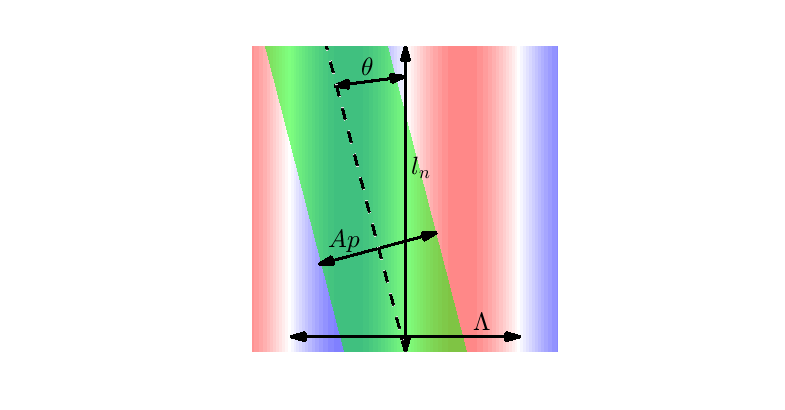
\includegraphics{../matlab/03_aero_optics_acoustics/planar_sample_domain.eps}
  \caption{General geometry for various sample calculations for showing the acoustic-optical coupling effect.}
  \label{fig:03_planar_sample_domain}
\end{figure}
For the following example, $l_n$ is the width of the acoustic disturbance (for example, the width of the wind tunnel), $\theta$ is the angle between the planar acoustic wave and the beam direction, $A_p$ is the aperture diameter of the beam, and $\Lambda$ is the wavelength of the acoustic wave.

Figure \ref{fig:03_planar_sample_calc_3} shows the time averaged $\opdrms$ per meter of beam propagation when the beam path is parallel ($\theta=0$) to the peaks and troughs of the planar acoustic wave as $\spl$ is varied.
\begin{figure}
  \centering
  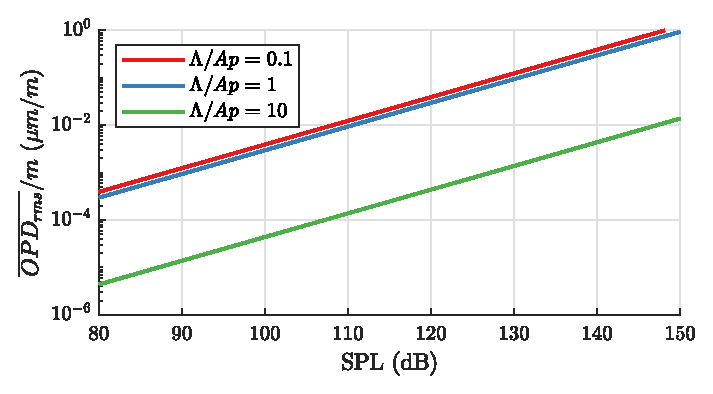
\includegraphics{../matlab/03_aero_optics_acoustics/planar_sample_calc_3.eps}
  \caption{Theoretical time-averaged $\opdrms$ per meter of beam propagation as a function of sound pressure level, $\spl$, for several $\Lambda/Ap$ ratios and $\theta=0$.}
  \label{fig:03_planar_sample_calc_3}
\end{figure}
As the sound pressure level increases the time averaged $\opdrms$ also increases and can easily reach the point of being a significant factor in the measured optical disturbance.
There is little difference between 0.1 and 1 $\Lambda/Ap$, but as the wavelength gets much larger compared to the beam diameter, then the optical effect of the noise is greatly reduced, this effect is known as aperture filtering \cite{Siegenthaler-2005-KQ2HGmfp}.

Aperture filtering is more clearly shown in Figure \ref{fig:03_planar_sample_calc_1}.
\begin{figure}
  \centering
  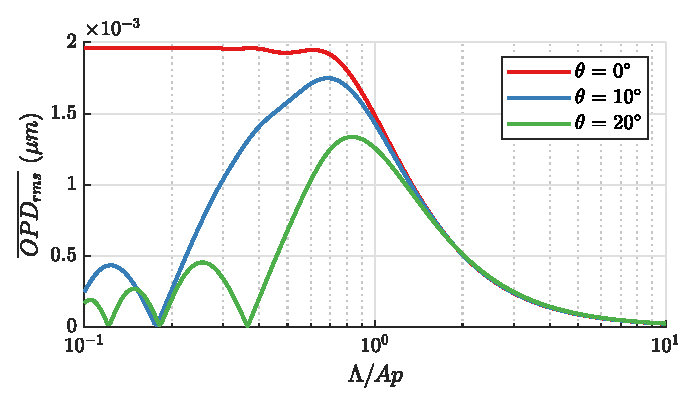
\includegraphics{../matlab/03_aero_optics_acoustics/planar_sample_calc_1.eps}
  \caption{Theoretical time-averaged $\opdrms$ for a rms sound pressure of 1 Pa ($\spl$ of 94 dB), $l_n$ of 1 m, and various angles and $\Lambda/Ap$ ratios.}
  \label{fig:03_planar_sample_calc_1}
\end{figure}
As the $\Lambda/Ap$ ratio increases from 0.1, time-averaged $\opdrms$ remains fairly constant until it starts to drop around $\Lambda/Ap$ of 0.7 and starts to asymptotically approach zero which it basically reaches by $\Lambda/Ap$ of 10.
Figure \ref{fig:03_planar_sample_calc_1} also shows the effect of changing the beam angle, $\theta$, through the acoustic field.
For nonzero $\theta$, the beam encounters alternating high and low index of refraction as it passes through the test region, so that the time-averaged $\opdrms$ begins to decrease compared to the $\theta = 0^\circ$ case below $\Lambda/Ap=1$.
There are also points of zero optical disturbance that occur at $\theta_{zero}=\tan^{-1}(n\Lambda/l_n)$ for $n\neq0$; these points occur because the peaks and valleys of the optical disturbance caused by the sound wave effectively cancel out over the length of the integration path, $l_n/\cos\theta$.

Figures \ref{fig:03_planar_sample_calc_3} and \ref{fig:03_planar_sample_calc_1} show the optical effect of plane acoustic waves in a no-flow environment.
The effect of wind-tunnel flow is to stretch (downstream-traveling waves) or compress (upstream-traveling waves) the wavelength of the acoustic noise thereby altering the filtering effect of the beam aperture.
Figure \ref{fig:03_planar_sample_calc_2} shows a typical optical disturbance from the two transverse acoustic waves (u+c and u-c) present in a wind tunnel at Mach 0.6.
\begin{figure}
  \centering
  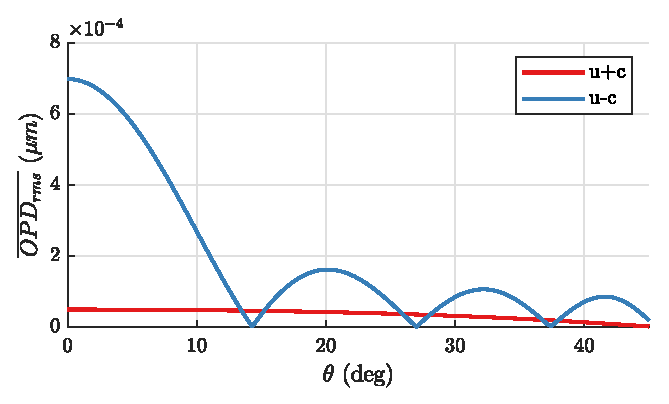
\includegraphics{../matlab/03_aero_optics_acoustics/planar_sample_calc_2.eps}
  \caption{Theoretical time-averaged $\opdrms$ for the two acoustic waves (u+c and u-c) for the blade pass frequency (534 Hz) at Mach 0.6 with a RMS sound pressure of 1 Pa ($\spl$ of 94 dB), $l_n$ of 1 m, and $Ap$ of 15 cm.}
  \label{fig:03_planar_sample_calc_2}
\end{figure}
Both waves have a RMS sound pressure of 1 Pa and the beam has an aperture of 15 cm and propagates through a 1 m acoustic field inside the tunnel.
Over a vast majority of the look back angles the upstream-traveling acoustic wave has a much greater effect on the optical disturbance compared to the downstream-traveling acoustic wave, due to the much shorter wavelength of the upstream-traveling waves which is less affected by aperture filtering.
However, the upstream-traveling wave goes through several zero points so the downstream-traveling wave dominates at some look back angles.

% In summary, Figures \ref{fig:03_planar_sample_calc_3} to \ref{fig:03_planar_sample_calc_2} give an example of how planar acoustic waves are expected to affect a beam traveling a finite distance $l_n$ at an angle $\theta$ through the acoustic field.

\subsection{Spherical Acoustic Waves}
The acoustic field from an speaker maybe assumed to be a spherical wave from a pulsating point if the frequency is sufficiently low and measurement region is far enough away from the source \cite{Randall-1951-9NtPPXPq}.
This pressure field when converted to complex pressure is represented by
\begin{equation}
  \hat{p}(r,t) = \frac{A_0}{r}\exp\left\{-j(kr-\omega t)\right\} \textrm{,}
  \label{eqn:03_spherical_pressure}
\end{equation}
where $A_0$ is the fluctuating pressure strength and $r$ is the distance from the source to the measurement point.
The RMS pressure of this field can be represented by
\begin{equation}
  p_{rms} = \frac{|A_0|}{r\sqrt{2}} \textrm{.}
  \label{eqn:03_spherical_pressure_rms}
\end{equation}

\subsubsection{Theoretical OPD Measurements}
A set of optical properties where calculated for a beam passing through a spherical acoustic field as defined by a point source using the process described previously in Chapter \ref{chap:03_simulated_beam}.
These calculations used an circular aperture size of 0.25-m in diameter consisting of 32x32 sub-apertures, an acoustic wavelength, $\Lambda$, of $Ap/4$ to $10Ap$, and a distance from the point source to the center of the aperture, $R$, of $5Ap$ to $25Ap$.
The beam was integrated over $\pm5$-m from the plane of the point source with 25 phase step used to calculate mean values.

The result of these simulated acoustic fields is shown in Figure \ref{fig:03_spherical_sample}.
\begin{figure}
  \centering
  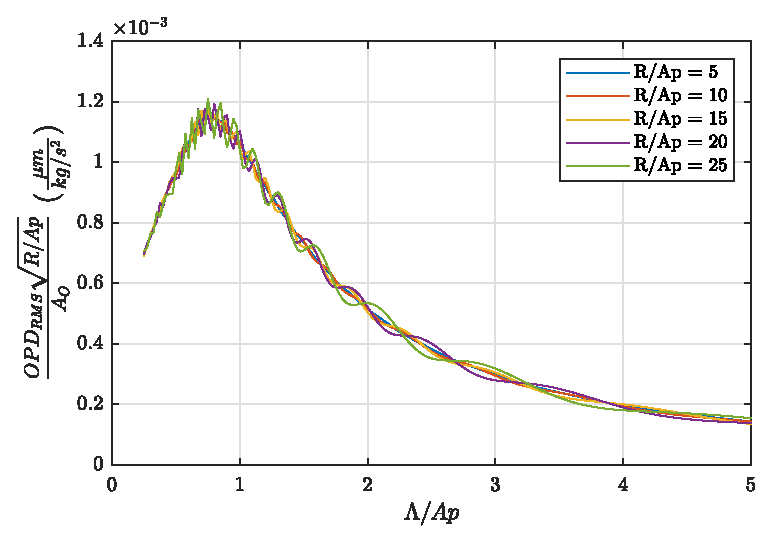
\includegraphics{../matlab/03_aero_optics_acoustics/spherical_sample.eps}
  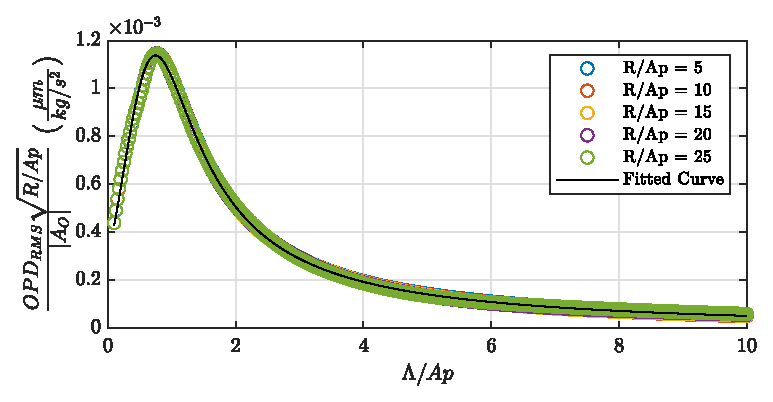
\includegraphics{../matlab/03_aero_optics_acoustics/spherical_sample_win.eps}
  \caption{Theoretical time-averaged $\opdrms$ for a spherical acoustic wave. The top plot shows a perfect spherical acoustic signal integrated over $\pm$5-m. The bottom plot shows has a Tukey window applied along the beam length to partially emulate source directivity which significantly reduces the measured oscillations.}
  \label{fig:03_spherical_sample}
\end{figure}
The top plots shows the expected optical disturbance ratio, $\opdrms/|A_0|$, for a perfectly spherical acoustic field measured over the beam length.
With the exception of some oscillations that are caused by end effects in the integration.
The oscillations can be greatly reduced by using a windowing function in the z-direction such as a Hanning or Tukey window which also can be used to roughly model directivity of the speaker's acoustic emission as shown in the bottom plot.
While this plot was calculated with a single aperture diameter, the general trend holds for all other aperture diameters that were tested, the only effect was the size and width of the oscillations.

The peak of the optical disturbance ratio, $\opdrms/|A_0|$, is located at $\Lambda/Ap\approx0.75$ for a circular aperture.
The signal is reduced above this value due to aperture filtering and below this value because the shorter wavelength have a reduced distance before alternating high and low index-of-refraction regions reduce the optical path difference.
When the acoustic source point is sufficiently far enough away from the measurement beam, $R/Ap\geq2$, the optical disturbance ratio, $\opdrms/|A_0|$ when multiplied by $\sqrt{R/Ap}$, can be collapsed onto a single curve for a range of $\Lambda/Ap$ of 0.1 to 10.
Above $\Lambda/Ap=10$ the curves start to diverge away from one another.
An approximate function fit to this data is
\begin{equation}
  \frac{\opdrms\sqrt{R/Ap}}{|A_0|} \approx \frac{p_1(\Lambda/Ap)^3+p_2(\Lambda/Ap)^2+p_3(\Lambda/Ap)+p_4}{(\Lambda/Ap)^3+q_1(\Lambda/Ap)^2+q_2(\Lambda/Ap)+q_3}
  \label{eqn:03_spherical_sample_fit}
\end{equation}
with coefficient values shown Table \ref{tab:03_spherical_sample_coeff}.
This functional fit has a $R^2$ value of 0.9991.
\begin{table}
\centering
\caption{Curve fit values for Figure \ref{fig:03_spherical_sample} and Equation \ref{eqn:03_spherical_sample_fit}}
\input{../matlab/03_aero_optics_acoustics/spherical_sample_win.txt}
\label{tab:03_spherical_sample_coeff}
\end{table}


\subsubsection{Measurement of a Spherical Acoustic Wave with an Optical Beam}
A small bench top experiment was used to compare the simultaneous optical and microphone measurements of an acoustic field from a speaker as shown in the measurement plane in Figure \ref{fig:03_speaker_test}.
\begin{figure}
  \centering
  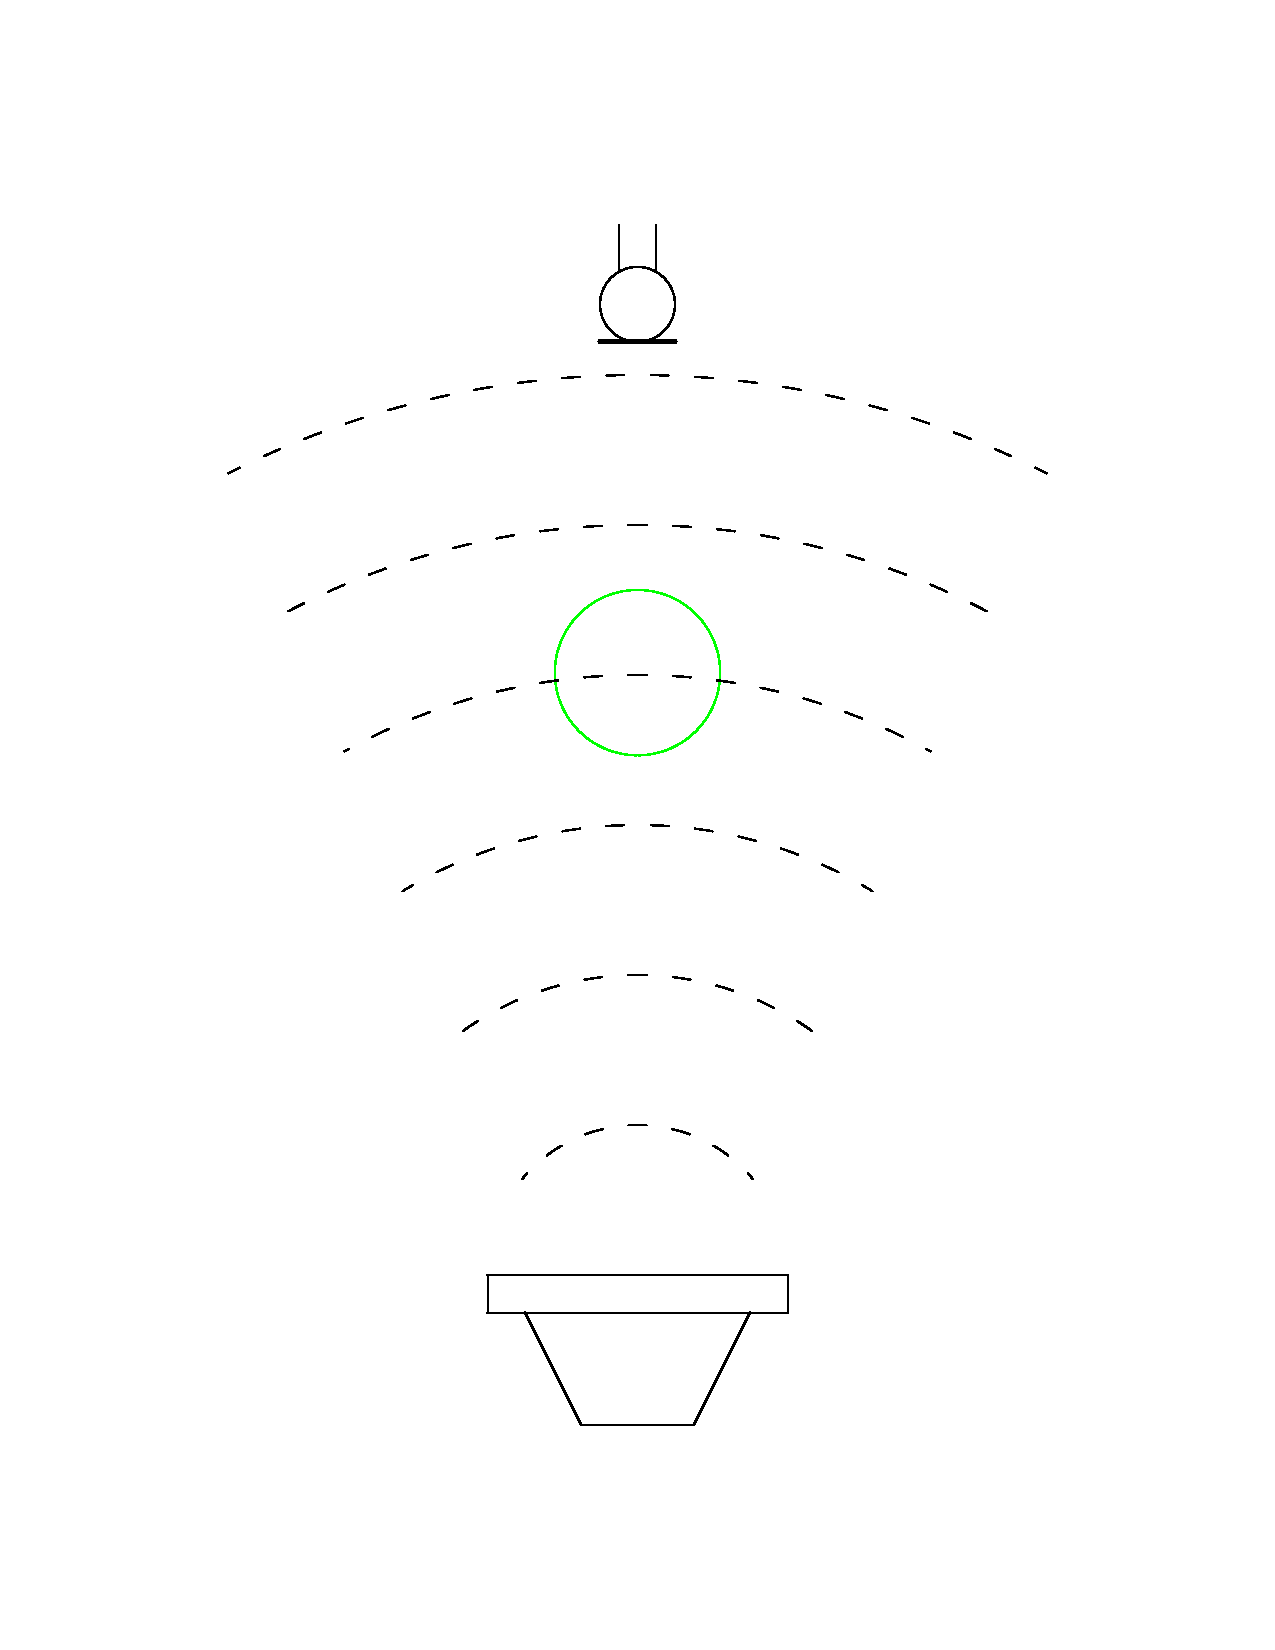
\includegraphics[width=3.5in,clip,trim=100 100 100 100]{../cad/speak_test.pdf}
  \caption{Spherical acoustic wave measurement test.}
  \label{fig:03_speaker_test}
\end{figure}
The distance from center of the beam to the speaker was 102-mm with a beam diameter of 28-mm.
An ACO model 7016B microphone \cite{ACO-Microphones} was placed directly over the speaker at a distance of 158-mm and was used with a Br\"uel \& Kj\ae r model 2670 preamplifier \cite{Bruel-Kjaer-2670}.
The speaker in use was Peerless model XT25SC90-04 \cite{Peerless-XT25SC90-04-1} which has a fairly flat on-axis response from 1-kHz to 40kHz.
% A Br\"uel \& Kj\ae r model 2690 \cite{Bruel-Kjaer-2690} signal conditioner was used as part of the data aquiztion system

The wavefront measurements system utilized in these measurements is similar to that shown in Figure \ref{fig:02_typical_wavefront_system} except there was no primary telescope.
The speaker was located in the center of the measurement region which was about 2-feet in length and the re-imaging telescope reduced the beam diameter by a factor of two and re-imaged the return mirror.
Optical wavefronts and microphone measurements were taken at 49-kHz.
The speaker was sinusoidally excited at three different frequencies (9, 14, and 18-kHz) at a variety of voltages.

The absolute value of the fluctuating pressure strength, $|A_0|$, was calculated two different ways.
The power spectra of the microphone data was used to calculate the average $p_{rms}$ at the excitation frequency and the fluctuating pressure strength using Equation \ref{eqn:03_spherical_pressure_rms}.
The optical wavefront was band-pass filtered at the excitation frequency using a process that will be discussed in Chapter \ref{chap:06}.
The time averaged $\opdrms$ was used to calculate the fluctuating pressure strength using Equation \ref{eqn:03_spherical_sample_fit}.

The results of these measurements of the fluctuating pressure strength is shown in Table \ref{tab:03_speherical_measurement}.
The differences between the two techniques for measuring the fluctuating pressure strength fell into two groups.
For the 9-kHz cases, the differences ranged from 20-26\% while the higher frequency cases the differences were between 1.1-1.5\% and in all cases the wavefront measurement reported a higher fluctuating pressure strength.
With the exception of the highest excitation case at 9-kHz, the differences between the to techniques was fairly constant for each frequency group.
Some of these differences maybe attributable to the frequency response of the microphone.
\begin{table}
  \centering
  \caption{Comparison of microphone and wavefront computation of $|A_0|$}
  \input{../matlab/03_aero_optics_acoustics/spherical_measurement.txt}
  \label{tab:03_speherical_measurement}
\end{table}

Measured and simulated wavefronts for the highest excitation cases at each frequency are shown in Figure \ref{fig:03_spherical_plot}.
\begin{figure}
  \centering
  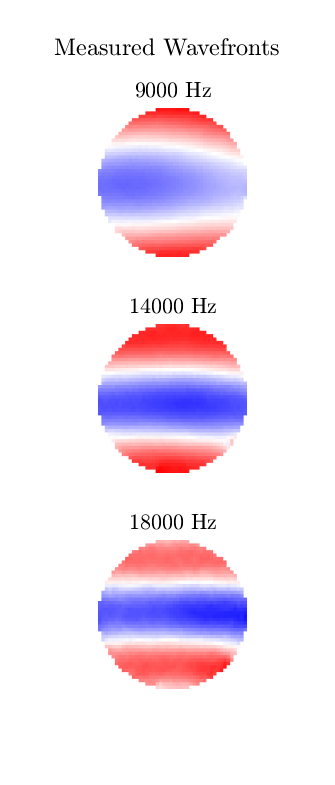
\includegraphics{../matlab/03_aero_optics_acoustics/spherical_plot_measured.eps}
  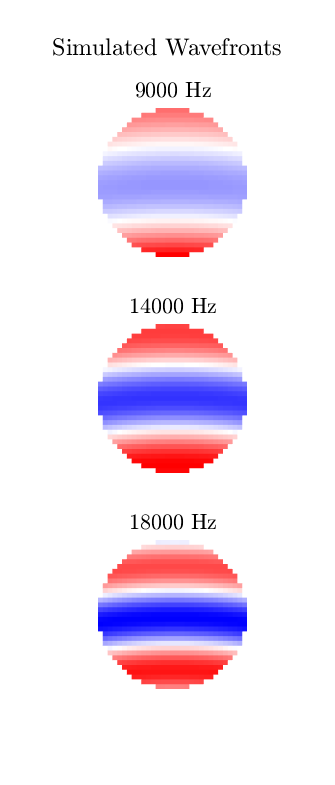
\includegraphics{../matlab/03_aero_optics_acoustics/spherical_plot_simulated.eps}
  \caption{Comparison of some of the measured wavefronts and simulated ones.}
  \label{fig:03_spherical_plot}
\end{figure}
The 9-kHz case shows some anomalies on the measured wavefront on the right side, diviating from spherical wave significantly likely contributing the significantly higher estimated pulsating field strength value when compared to the microphone estimate.
The 14 and 18-kHz cases show some remarkable agreement between the measured and simulated images.
Optical wavefront measurements can be utilized for making non-intrusive acoustic field measurements espically when the acoustic field is simple.



\section{Estimating the Acoustic Field Inside the Test-Section}



\subsection{Mode Marching Process}
\begin{enumerate}
  \item Start with a known or assumed source acoustic field, $p^n(x,y)$

  \item Calculate the transmitted pressure ratio
  \begin{itemize}
    \item Traveling with subsonic flow
      \begin{equation}
        \frac{p^t}{p^i} = \left(\frac{1+M_n}{1+M_{n+1}}\right)\left(\frac{2M_{n+1}}{M_n+M_{n+1}}\right)\left(\frac{X_{n,n}}{X_{n,n+1}}\right)\left(\frac{X_{n,n}}{X_{n+1,n+1}}\right)^{1/(\gamma-1)}
      \end{equation}
    \item Traveling against subsonic flow
      \begin{equation}
        \frac{p^t}{p^i} = \left(\frac{1-M_n}{1-M_{n+1}}\right)\left(\frac{2M_{n+1}}{M_n+M_{n+1}}\right)\left(\frac{X_{n,n}}{X_{n,n+1}}\right)\left(\frac{X_{n,n}}{X_{n+1,n+1}}\right)^{1/(\gamma-1)}
      \end{equation}
    \item Where
      \begin{equation}
        X_{a,b} = 1+\frac{\gamma-1}{2}M_aM_b
      \end{equation}
  \end{itemize}

  \item March acoustic field to next axial step,
    \begin{equation}
      p^{n+1}(x,y) = p^{n}(x,y)\frac{p^t}{p^i}\exp\{j(\omega t\mp k_{zm}^\pm z)\}
    \end{equation}

  \item Best-fit set of local duct modes coefficients, $C_m$, to acoustic field $p^{n+1}(x,y)$

  \item Calculate new acoustic field from duct mode and repeat from step 2
    \begin{equation}
      p^n(x,y) = \sum_{m=0}^{M} C_m\cdot p_m(x,y)
    \end{equation}

  \item When the end point is reached, step inlet acoustic field (rotate fan) and repeat
\end{enumerate}
